\setAuthor{}
\setRound{piirkonnavoor}
\setYear{2019}
\setNumber{G 6}
\setDifficulty{6}
\setTopic{TODO}

\prob{Kondensaator}
\begin{wrapfigure}[6]{r}{0.30\textwidth}
\vspace{-45pt}
	\begin{center}
		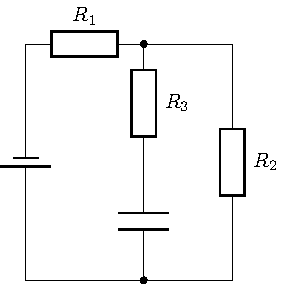
\includegraphics[width = 0.30\textwidth]{2019-v2g-06-yl.pdf}
	\end{center}
\end{wrapfigure}


Kondensaatorit laetakse kõrvaloleva skeemi järgi alalisvooluallikast pingega $U=\SI{12}{\V}$. Skeemis olevate takistite takistused on vastavalt $R_1=\SI{1}{\kilo\ohm}$, $R_2=\SI{2}{\kilo\ohm}$ ning $R_3=\SI{3}{\kilo\ohm}$. Leida maksimaalne pinge, milleni saame kondensaatori niimoodi laadida. 
\vspace{10pt}

\hint

\solu
Pinge kondensaatoril on  maksimaalne, kui see on täis laetud \pp{1}. Sellisel juhul kondensaatorit ning ka takistit $R_3$ vool ei läbi \pp{1} ning omakorda pingelang takistil $R_3$ on null \pp{1}. See tähendab, et pinge kondensaatori klemmidel on võrdne pingega takistil $R_2$. \pp{2} Viimase saamegi leida Ohmi seadusest:
$$U_2=I_2R_2 \quad I_2=\frac{U}{R_1+R_2} \Rightarrow U_2=U_C=\frac{U}{R_1+R_2}R_2\quad\pp{2}$$
Asendame sisse teada olevad väärtused:
$$U_C=\frac{\SI{12}{\V}}{\SI{1}{\kilo\ohm}+\SI{2}{\kilo\ohm}}\cdot\SI{2}{\kilo\ohm}=\SI{8}{\V}\quad\pp{1}$$
\probend